
\chapter{Supplementary Material of ``Mean-field predictions of scaling prefactors match low-dimensional jammed packings''}
\author{James D Sartor, Sean A. Ridout, Eric I. Corwin}
%\affiliation{$^*$Department of Physics and Materials Science Institute, University of Oregon, Eugene, Oregon 97403, USA \\ $^\dagger$Department of Physics and Astronomy University of Pennsylvania, Philadelphia, PA 19104, USA}
%\maketitle

\label{excessContactsScalingSupplement}
%\onecolumn

\subsection{Measured values of $\varphi_j$}
In Table \ref{table:phij} we show our measued values of $\varphi_j$. these values are used in calculating $\Delta \varphi$.

\begin{table}[ht]
\caption{Measured values of $\varphi_j$ in dimensions 2-10.
\label{table:phij}}
\begin{tabular}{ |c|c|c|c|c|c|c|c|c|c| } 
 \hline
 d & 2 & 3 & 4 & 5 & 6 & 7 & 8 & 9 & 10 \\ 
 \hline
 $\varphi_j$ & 0.85 & 0.65 & 0.46 & 0.31 & 0.20 & 0.13 & 0.078 & 0.049 & 0.029\\ 
 \hline
\end{tabular}
\end{table}

\section{Mean Field Predictions of Prefactors}

\subsection{Mean Field Prediction of Pressure vs Packing Fraction}

Mean field theory predicts that pressure scales with packing fraction as follows \cite{parisi_theory_2020}:
\begin{align}
 \hat{P} &= \hat{C}(\hat{\varphi} - \hat{\varphi}_j) \label{sup_eqn:pvsphi}
 \end{align}
 where $\hat{C}_{p\varphi}$ is a constant, and the hats over $P$ and $\Delta \varphi$ signify that the quantities are scaled such to be fixed in the infinite dimensional limit, as follows:
 \begin{align}
\hat{P} &= \frac{P^*}{\rho d} \label{sup_eqn:phat} \\
\hat{\varphi} &= \frac{2^d}{d} \varphi %= \frac{\bar{V_p}}{d} \rho
 \end{align}
where $\rho$ is the number density, $\frac{N}{V}$, and $P^*$ is the pressure which is calculated with assumed unit particle diameter. This relates to our pressure, $P$, as follows:
\begin{align}
 P & = \frac{\varphi}{\rho} \frac{1}{d^2} P^* \label{sup_eqn:pstar} , 
\end{align}
where the factor of $\frac{\varphi}{\rho}$ unwraps their assumption of unit particle diameter, and the factor of $\frac{1}{d^2}$ comes from their potential, which explicitly contains a dimensional term:
\begin{align}
 U^*(r) &= \frac{\epsilon d^2}{2} \left(\frac{r}{\ell}-1\right)^2 \Theta\left(\ell-r\right).
\end{align}
We can thus rewrite equation \ref{sup_eqn:phat} in terms of our pressure $P$:
\begin{align}
 \hat{P} &= \frac{d}{\varphi}P,
\end{align}
 and therefore equation \ref{sup_eqn:pvsphi}:
 \begin{align}
  \frac{d}{\varphi}P &=\hat{C}\frac{2^d}{d}( \varphi - \varphi_j) \\
  P &= \frac{\varphi}{d} \hat{C} \frac{2^d}{d} \Delta \varphi \\
  P &= \frac{1}{d}\hat{C}\hat{\varphi}_j( \Delta \varphi) \\
   P &= \frac{1}{d}\hat{C}_{p\varphi}( \Delta \varphi). \label{sup_eqn:finalpvsphi}
\end{align}
%
Where, noting that $\hat{\varphi}_j$ and $\hat{C}$ are constants in the infinite dimensional limit, we combine them as $\hat{C}_{p\varphi}$. Thus mean field predicts a simple $1/d$ scaling of the prefactor between pressure and excess packing fraction.


\subsection{Mean Field Prediction of Pressure vs Number Of Excess Contacts}

The number of contacts, $z$, is predicted by mean field theory to have the form \cite{parisi_theory_2020}:
%
\begin{align}
\frac{z}{2d} &=1 + \hat{C}_{z\varphi}\sqrt{\hat{\varphi}-\hat{\varphi_j}} \\
\frac{z}{2d} &=1 + \hat{C}_{z\varphi}\sqrt{\frac{2^d}{d}}\sqrt{\varphi-\varphi_j} \label{eqn:meanFieldExcessPhi}
\end{align}
%
for some constant $\hat{C}_{z\varphi}$. 

The number of excess contacts, $\delta z$, therefore is predicted to scale as follows:
\begin{align}
\frac{\delta z}{2d} &= \hat{C}_{z\varphi}\sqrt{\frac{2^d}{d}}\sqrt{\varphi - \varphi_j} \\ % the 1 goes away cuz it's dz
\delta z &= 2d\hat{C}_{z\varphi}\sqrt{\frac{2^d}{d}}\sqrt{\varphi - \varphi_j} \label{supeqn:finalphivsz}.
\end{align}


\subsection{Mean Field Prediction of Packing Fraction vs Number of Excess Contacts}

By combining equations \ref{sup_eqn:finalpvsphi} 
and \ref{supeqn:finalphivsz},
we can also predict the relation between $\delta z$ and $P$:
%
\begin{align}
 \delta z &= 2d\hat{C}_{z\varphi}\sqrt{\frac{2^d}{d}} \sqrt{\frac{d}{\hat{C}_{p\varphi}}P} \\
 &= 2d\hat{C}_{z\varphi}\sqrt{\frac{2^d}{\hat{C}_{p\varphi}}} \sqrt{P} \\
\end{align}
%
where we define $\hat{C}_{zp}=\frac{2\hat{C}_{z\varphi}}{\sqrt{\hat{C}_{p\varphi}}}$.

\begin{figure}[th!]
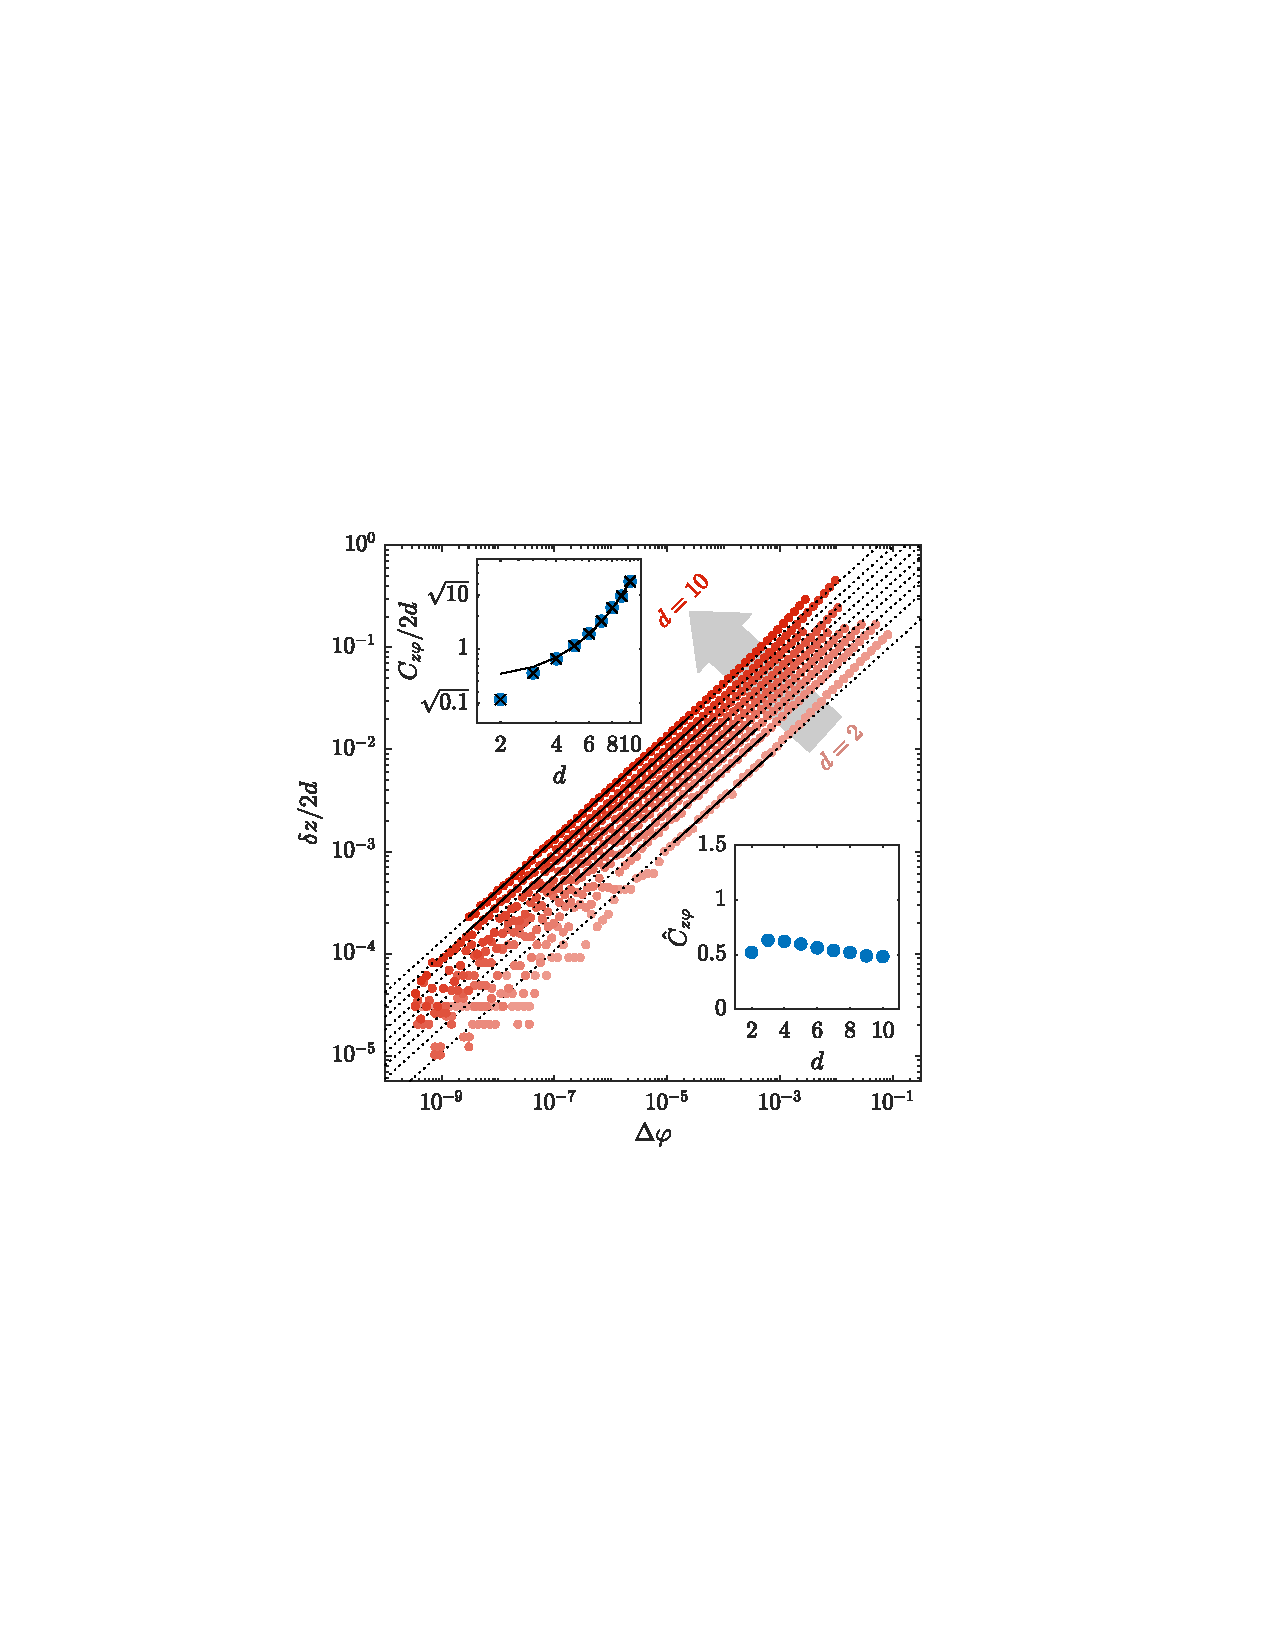
\includegraphics[width=300px, trim=143 240 168 250, clip]{excessContactsScaling/evsphi.pdf}

\caption{Measured excess contacts scales with the square root of excess packing fraction for systems from $d=2$ to $d=10$ (red circles). Black lines show the fits for $C_{zp}$ using eqn \ref{eqn:evsphi}. For our fits, we ignore data at high pressure and low contact number as in figure \ref{plot:evsp}.
Dotted lines show the extension of our fits beyond the fitted range. Inset shows the measured values of $C_{z\varphi}$ (blue circles), which scale in agreement with the mean field prediction eqn \ref{supeqn:finalphivsz} using measured values of with $\hat{C}_{z\varphi} \approx 0.83$. Additionally, to note consistency we show that our measured values of $C_{z\varphi}$ agree well with values calculated from our measurements of $C_{p\varphi}$ and $C_{zp}$ using eqn \ref{eqn:consistency} (black x's).}

\label{plot:evsphi}
\end{figure}
%
\subsection{Excess Contacts vs Excess Packing Fraction Prefactor Scaling}

From eqns \ref{eqn:pvsphi} and \ref{eqn:evsp} 
we can simply relate $\delta z$ and $\varphi$ as follows:
%
\begin{equation}
\delta z=C_{z\varphi}\left(\Delta\varphi\right)^{1/2} \label{eqn:evsphi}
\end{equation}
%
where clearly, 
\begin{align}
C_{z\varphi}=C_{zp}\sqrt{C_{p\varphi}}. \label{eqn:consistency}
\end{align}

In figure \ref{plot:evsphi}, we show this scaling seperately for each dimension. We fit each line to eqn \ref{eqn:evsphi} to find the values of the prefactor $C_{z\varphi}$ in each dimension, the values of which are shown in the inset. These values agree well with both the mean field prediction above $3D$, shown as a black line, and our calculated value from $C_{zp}$ and $C_{p\varphi}$, shown as black x's in figures \ref{plot:pvsphi} 
and \ref{plot:evsp}.

%
\subsection{Dimensional Dependence of Force Moment Ratios}
In figure \ref{plot:mfr} we show that the ratio of force moments does not depend strongly on dimension. This empirical fact may seem at odds with previous reports of how the low-force part of the distribution differs from its mean-field form in low dimensions \cite{charbonneau_jamming_2015,mueth_force_1998}. The low-force part of the distribution has $P(f) \propto f^\theta$, where $\theta\approx 0.17$ in $d=2$ smoothly rises to a $d=\infty$ value of $\theta \approx 0.42$. The high-force behaviour decays like an exponential or a stretched exponential; thus, we have computed the theoretical value of this moment ratio for distributions of the form $P(f) \sim f^\theta e^{-f /f_0}$ and $P(f) \sim f^\theta e^{-f^2 /f_0^2}$, as shown in figure \ref{plot:theory_mfr}. We find that neither of these assumed distributions quantitatively predicts the measured moment ratio for the known values of $\theta$, but they do show that the known variation in $\theta$ should not make us expect a large variation in this moment ratio.



\begin{figure}[h!]
%    \caption{Dimensional dependence of force moment ratios}
%  \label{plot:test}
%  \begin{subfigure}[t]{0.47\columnwidth}
  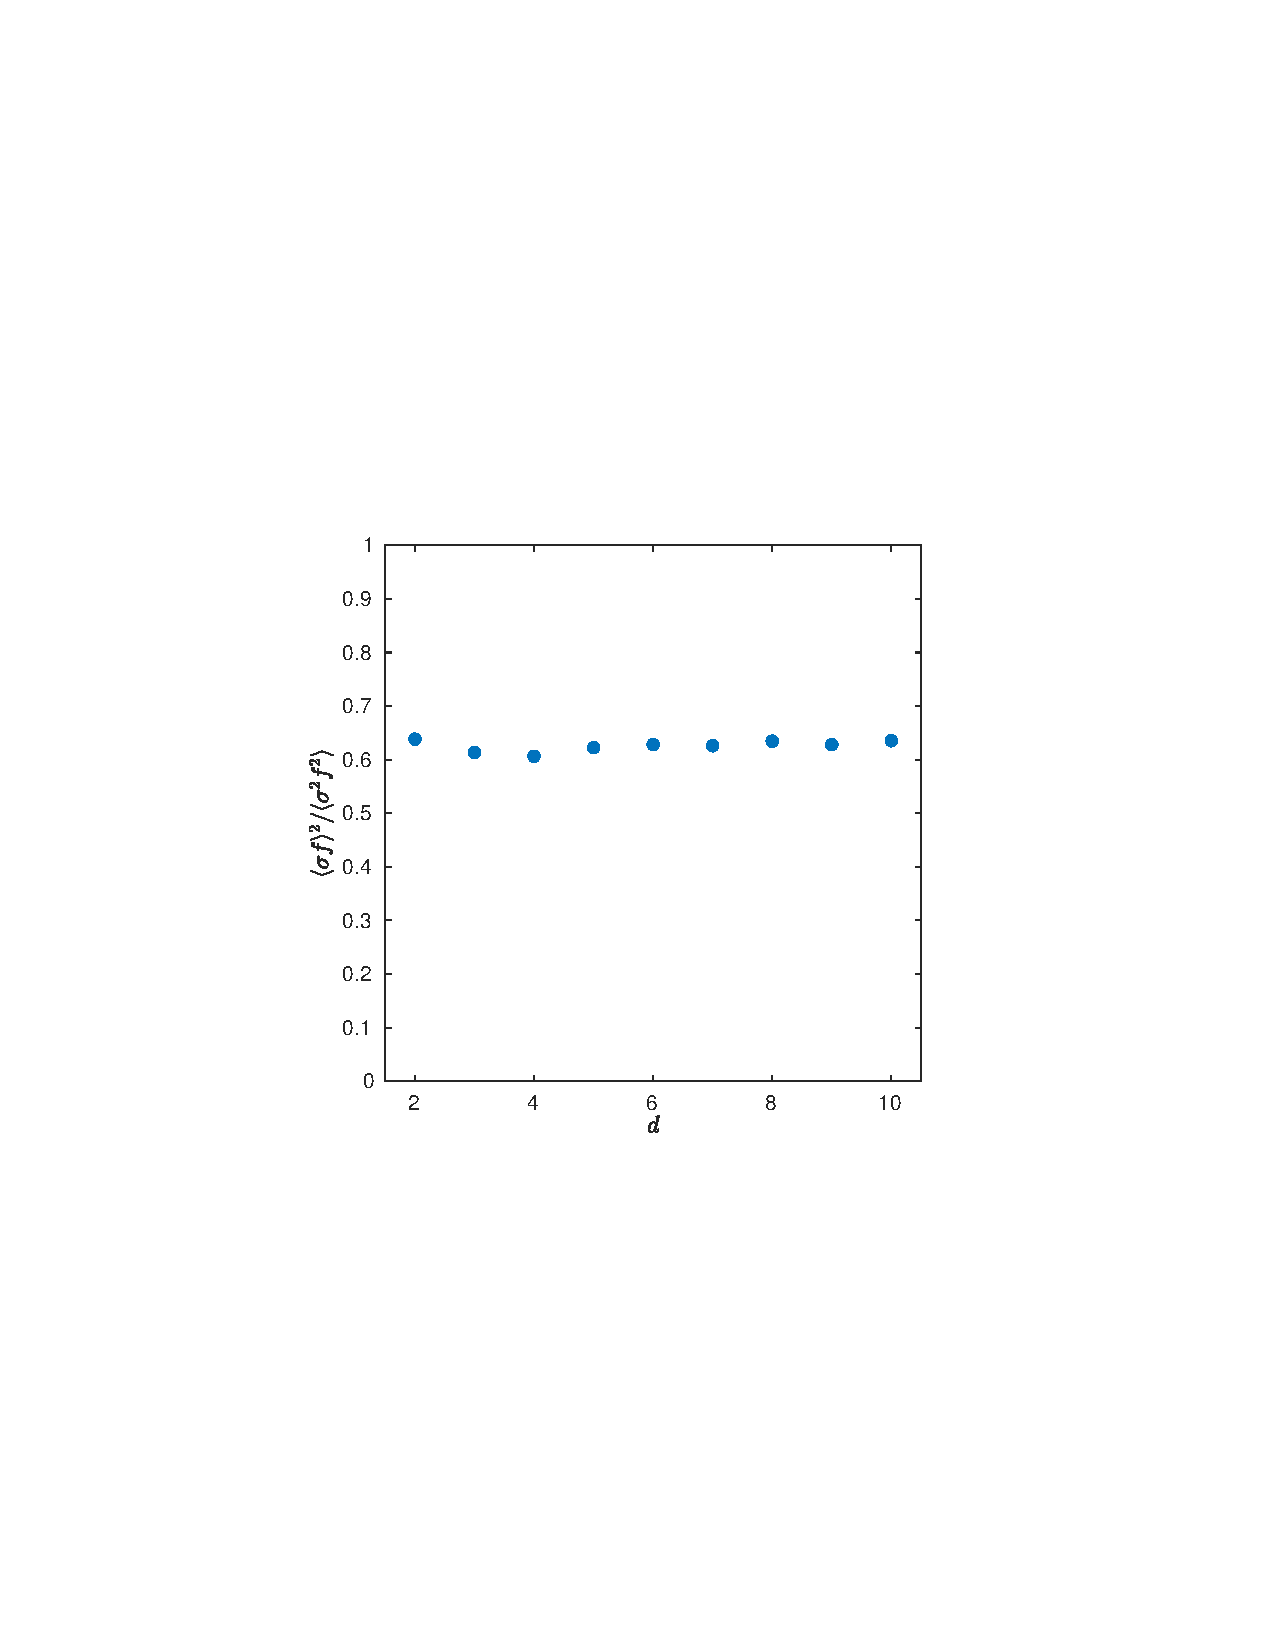
\includegraphics[width=230px, trim=133 242 168 254, clip]{excessContactsScaling/mfr.pdf}
     \caption{Dimensionless moment ratio of first and second moments of $\sigma f$ shows no dimensional dependence}
     \label{plot:mfr}
\end{figure}
\begin{figure}[h!]
     %  \end{subfigure}
%  \hfill %%
%  \begin{subfigure}[t]{0.47\columnwidth}
    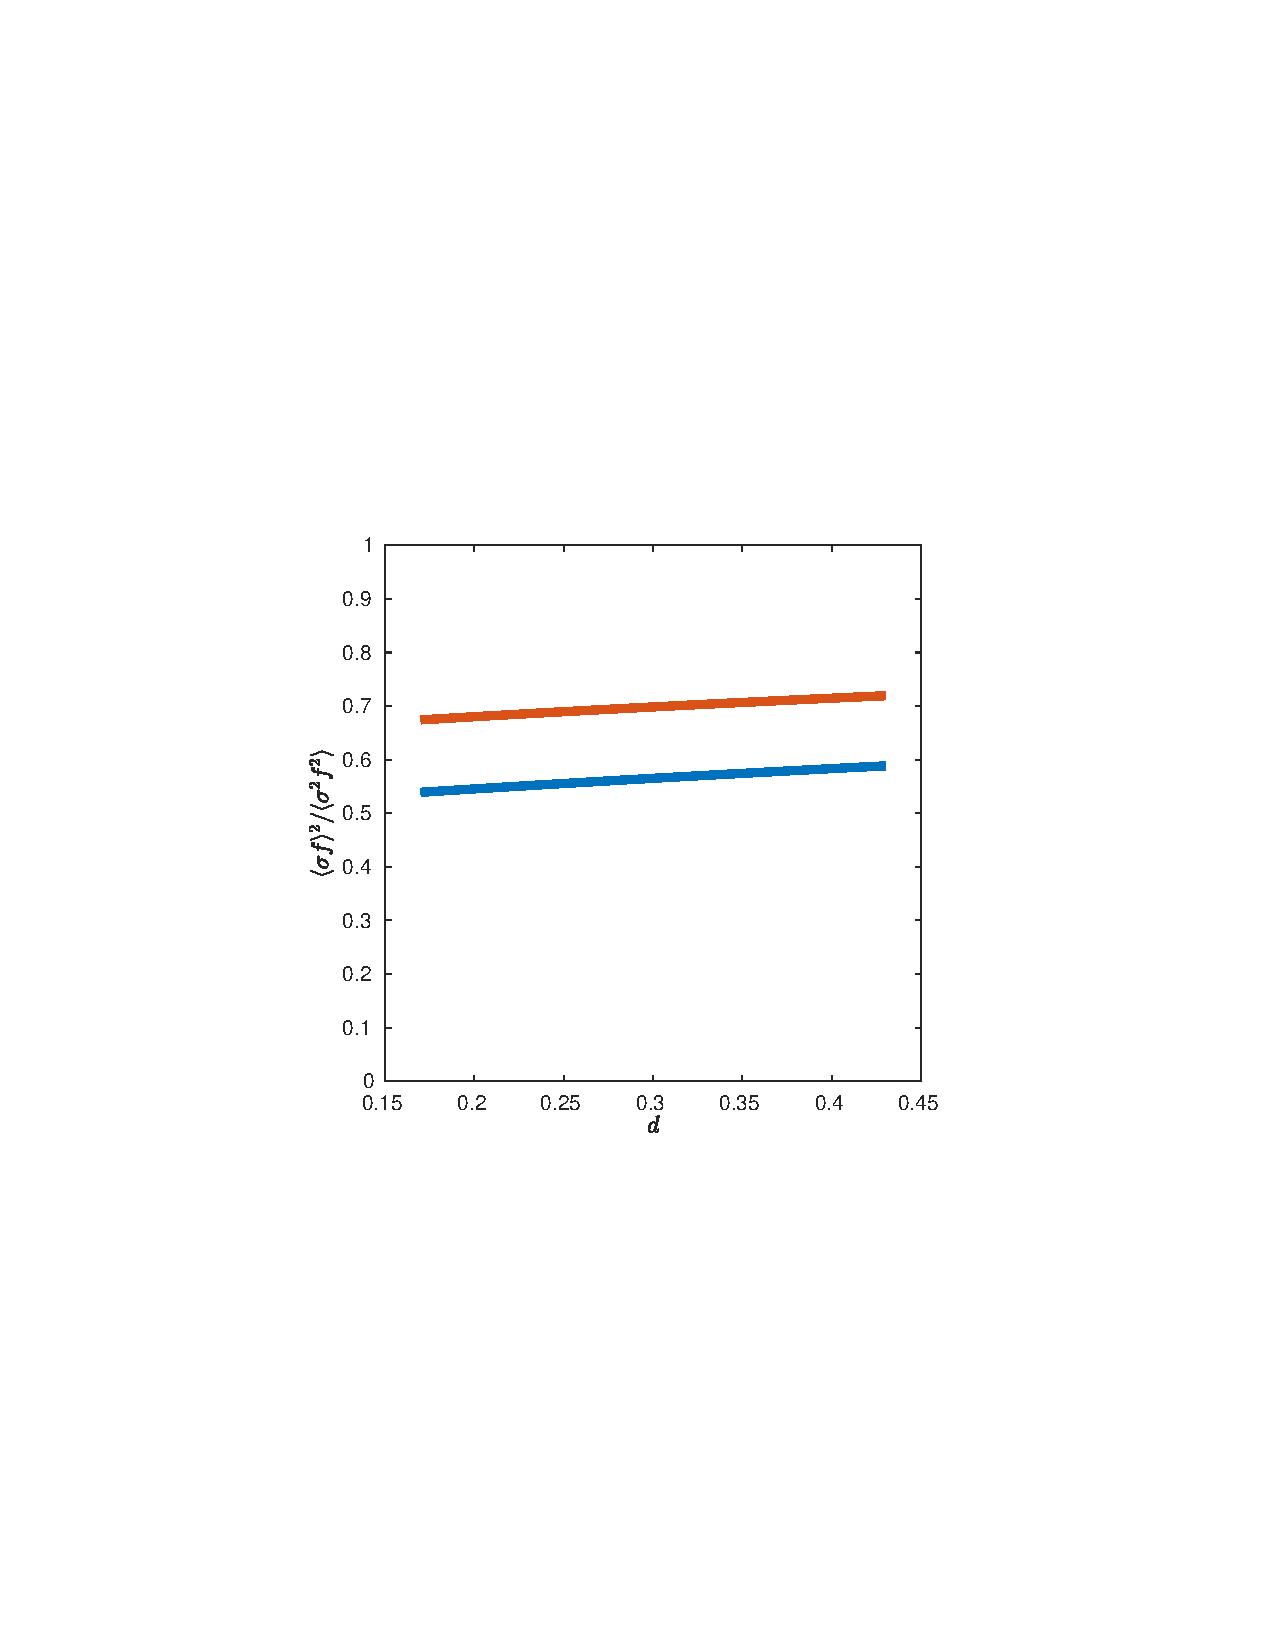
\includegraphics[width=230px, trim=143 240 163 250, clip]{excessContactsScaling/theoryMFR.pdf}
    \caption{Neither the force distribution $f^\theta e^{-f/f_0}$  (blue) nor the distribution $f^\theta e^{-f^2/f_0^2}$  (red) predicts a strong $\theta$ dependence for the relevant moment ratio}
    \label{plot:theory_mfr}
%  \end{subfigure}
\end{figure}




\subsection{Accounting for Polydispersity in Pressure vs. Packing Fraction Scaling}

To account for the case with varying spring constants we also form the matrix of inverse spring constants

\begin{equation}
k^{-1} = \frac{1}{2 \eps} \mqty(\dmat{\sigma^2_{ij},\ddots,\sigma^2_{kl}}). \label{eqn:compliance}
\end{equation}

and the projection operator onto the states of self stress

\begin{equation}
S = \sum_{i=1}^{N \Delta z} \ket{s_i}\bra{s_i}.
\end{equation}

In terms of these quantities, the bulk modulus may be written as \cite{pellegrino_structural_1993, wyart_rigidity_2005, lubensky_phonons_2015}

\begin{equation}
\pdv[2]{E}{V} = \frac{1}{V}  \bra{E} S  \left(S \left(k^{-1}\right) S \right)^{-1} S \ket{E}. \label{eqn:genf}
\end{equation}

In the one SSS approximation, we can evaluate the two projected quantities that we need to evaluate equation \ref{eqn:genf}. Equations \ref{eqn:affine} 
and \ref{eqn:sss} 
give

\begin{align}
    S \ket{E} = \bra{s_0}\ket{f} \ket{s_0}= \frac{\bra{r}\ket{f}}{d \sqrt{\bra{f}\ket{f}}}\ket{s_0} = \sqrt{Z}\frac{\langle r f \rangle}{d \sqrt{\langle f^2 \rangle}} \ket{s_0}, 
\end{align}

and equations \ref{eqn:compliance} and \ref{eqn:sss} 
give

\begin{align}
    S k^{-1} S &= \ket{s_0} \mel{s_0}{k^{-1}}{s_0} \bra{s_0} =  \ket{s_0}\frac{\langle \sigma^2 f^2 \rangle}{2 \epsilon \langle f^2 \rangle} \bra{s_0}\\
    \left(S k^{-1} S\right)^{-1} &= \ket{s_0}\frac{2 \epsilon\langle f^2 \rangle}{\langle \sigma^2 f^2 \rangle} \bra{s_0}
\end{align}

Furthermore at lowest order in $P$ we have $\ket{r} = \ket{\sigma}$, and we may assume $Z \approx d N$. Thus, equation \ref{eqn:genf} reduces to 

\begin{equation}
K = \frac{2 N \eps}{ d V}  \frac{\langle \sigma f \rangle^2}{\langle \sigma^2 f^2 \rangle},
\end{equation}

and thus via equation \ref{eqn:CisK}:

\begin{equation}
    C_{p\varphi} = \frac{2}{d} \frac{ \langle \sigma f \rangle^2}{\langle \sigma^2 f^2 \rangle}.\label{eqn:seanPredictionSupp}
\end{equation}

\subsection{Prestress Comparison}

It has recently been suggested the relationship between prestress and number of excess contacts collapses perfectly when compared across dimensions \cite{shimada_low-frequency_2019}. We define prestress $e$ as in ref. \cite{shimada_low-frequency_2019} as:
%
\begin{align}
 e = \left(d-1\right) \left\langle \frac{-V'(r_{ij})}{r_{ij}V''(r_{ij}} \right\rangle_{ij}
\end{align}
%
and expected to scale as:
%
\begin{align}
 \delta z &= C_{ze} e^\frac{1}{2} \label{sup_eqn:evsprestress}
\end{align}
%
because it is proportional to pressure near the jamming transition \cite{shimada_low-frequency_2019}. In figures \ref{plot:evsprestress} and  \ref{plot:evspcomp},, we examine the collapse of scaled excess contacts with prestress and compare it to the collapse of excess contacts scaled by the mean field prediction with pressure. In figure \ref{plot:evsprestress} we see that the collapse with prestress is not quite perfect - there is a clear upward trend. This stands in contrast to the inset of figure \ref{plot:evspcomp}, which shows $\hat{C}_{zp}$ to be nearly constant above three dimensions.


  
\begin{figure}[h!]
 %   \caption{Comparison of scaled excess contacts with pressure and prestress.}
% \label{plot:comparison}
% \begin{subfigure}[t]{0.47\columnwidth}
    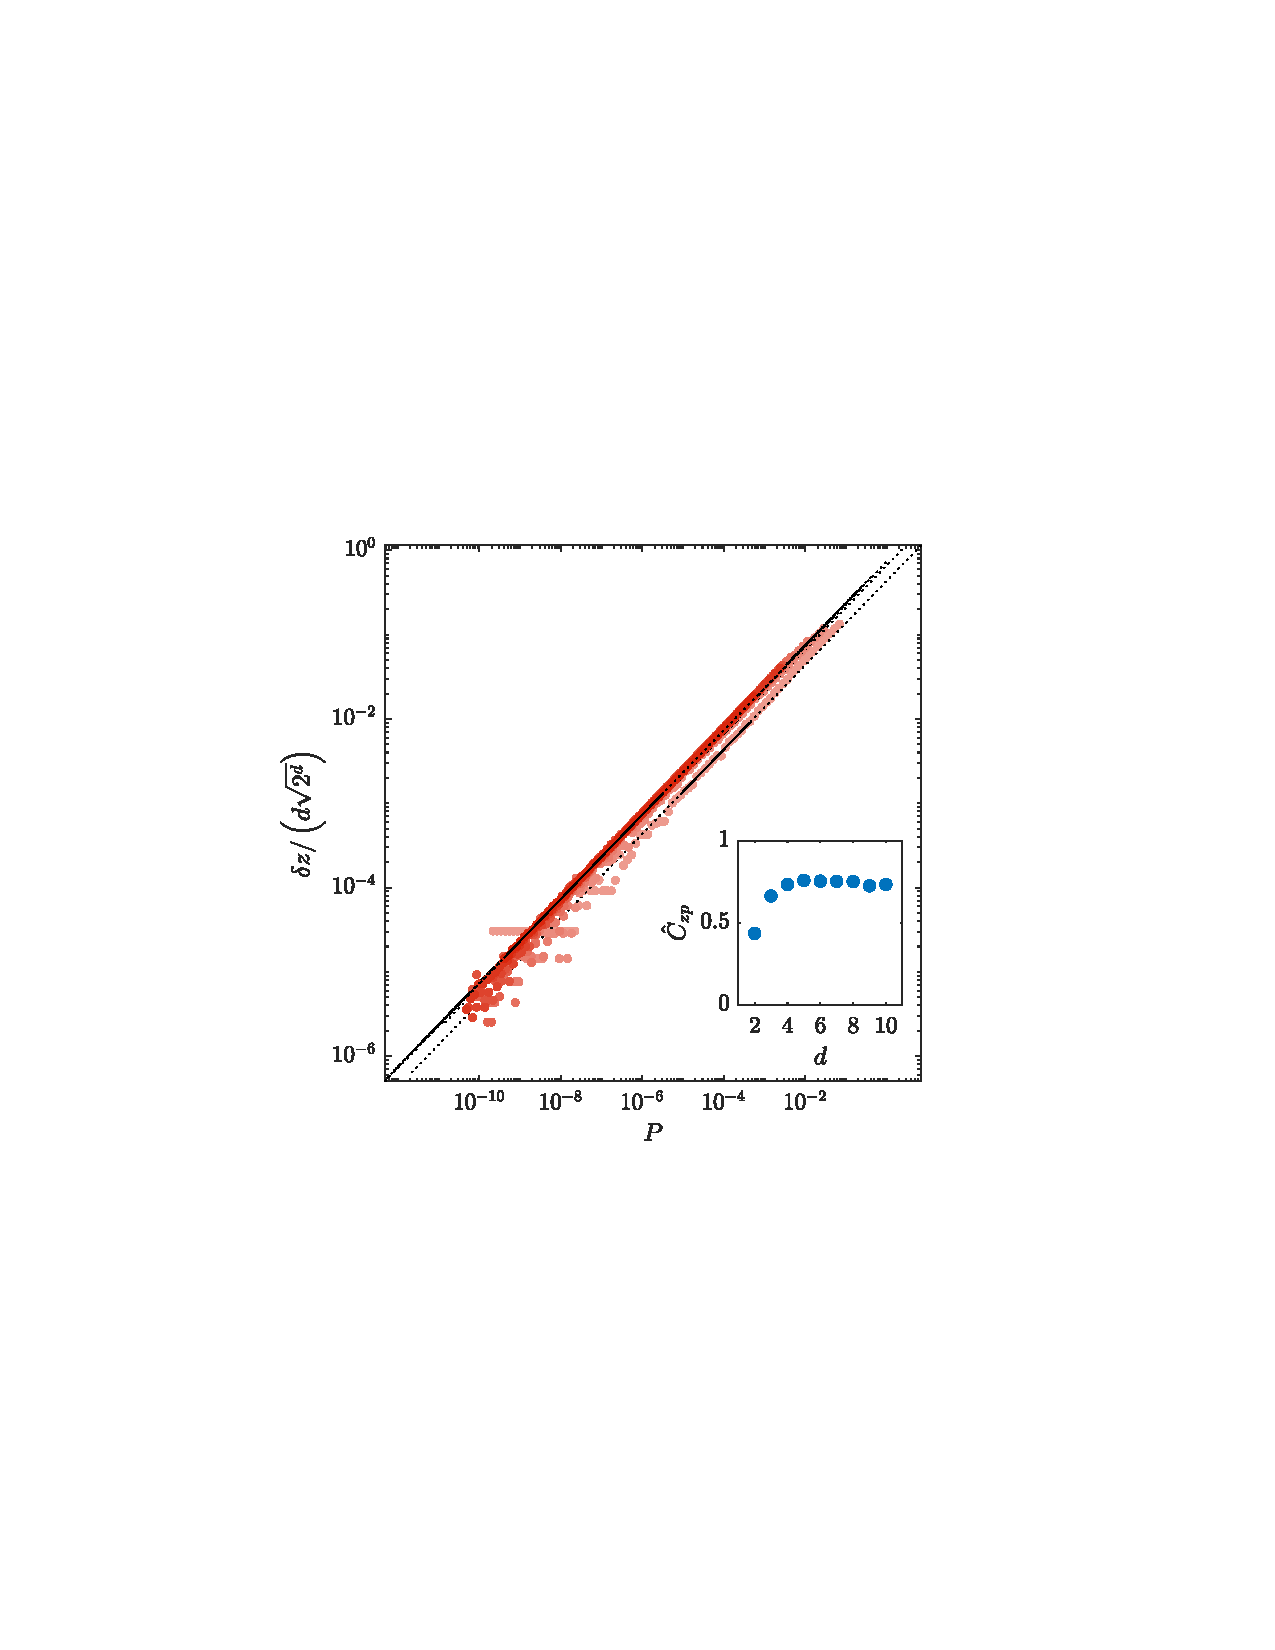
\includegraphics[width=230px, trim=133 242 168 254, clip]{excessContactsScaling/evspcomp.pdf}
   \caption{Scaled excess contacts scales with the square root of pressure as in figure \ref{plot:evsp}. 
    However, with excess contacts scaled by the expected mean field prediction, eqn. \ref{eqn:meanFieldExcessPressure},
    the data collapse onto a single line. The inset confirms the collapse, showing $\hat{C}_{zp}$ to be nearly constant.}
     \label{plot:evspcomp}
\end{figure}
\begin{figure}[h!]
%  \hfill %%
%  \begin{subfigure}[t]{0.47\columnwidth}
    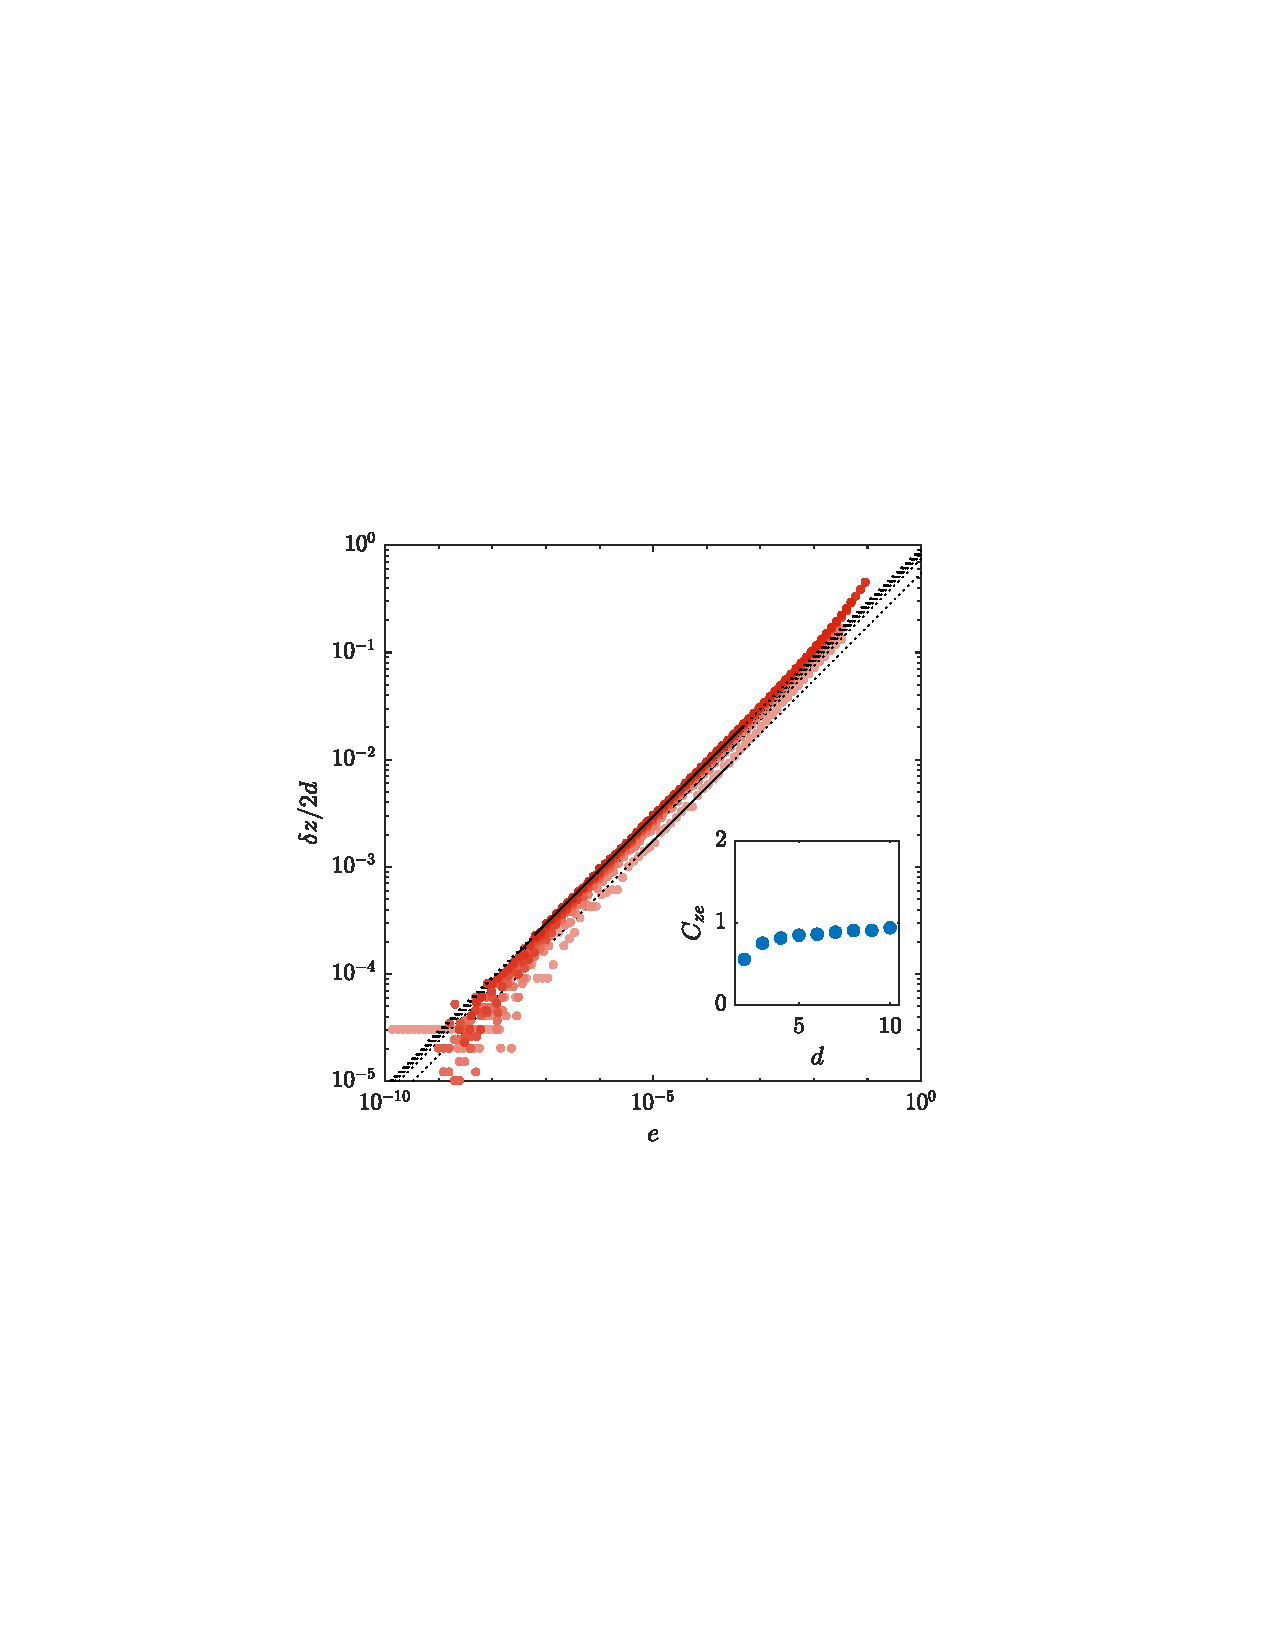
\includegraphics[width=230px, trim=143 240 163 250, clip]{excessContactsScaling/prestressvse.pdf}
    \caption{Scaled excess contacts scales with the square root of prestress for systems from $d=2$ to $d=10$. Black lines show the fits for $C_{ze}$ using eqn \ref{sup_eqn:evsprestress}. The fits ignore high and low pressure data as in figure \ref{plot:evsp}. 
    Lower inset shows the measured values of $C_{ze}$ which have a clear upward trend.}
    \label{plot:evsprestress}
%  \end{subfigure}
\end{figure}

In fact, close to jamming so that $r \approx \sigma$ and $Z \approx N d$, our dimensionless pressure $P$ as defined in equation \ref{eqn:stress_tensor_definition}  
is related to the prestress by
%
\begin{align} P &= \frac{\bar{V}_p}{\varepsilon Vd} \sum_{i,j} \mathbf{f}_{ij} \cdot \mathbf{r}_{ij} \\
  &=\frac{\bar{V}_p}{\varepsilon Vd} Z \langle f_{ij} r_{ij} \rangle_{ij} \\
  &=\frac{2 \varphi Z}{ d}  \left\langle \frac{r_{ij}}{\sigma_{ij}} \left(1 - \frac{r_{ij}}{\sigma_ij}\right) \right\rangle_{ij}\\
  &= \frac{2 \varphi Z}{d}  \left\langle \frac{- r_{ij} V'(r_{ij})}{\sigma_{ij}^2V''(r_{ij}} \right\rangle_{ij} \\
&\approx 2\frac{ \varphi_{\mathrm{J}} }{d-1} e.
\end{align}
%
Thus, our better-fitting form for the $z-P$ relationship amounts to the statement that
%
  \begin{equation}
    \frac{\Delta z}{2 d} =  \hat{C}_\varphi   \sqrt{\frac{d}{d-1}} \sqrt{e}.
  \end{equation}
%
 Thus our scaling forms agree with the statement of reference \cite{shimada_low-frequency_2019} in the infinite-$d$ limit, although we see better fit with our form in low dimensions.


%\bibliography{scaling}% Produces the bibliography via BibTeX.

%\end{document}
%yes
% ****** End of file aipsamp.tex ******

